\documentclass[11pt, a4paper]{article}
\usepackage{pdfpages}
\usepackage{parallel}
\usepackage[T2A]{fontenc}
\usepackage{ucs}
\usepackage[utf8x]{inputenc}
\usepackage[polish,english,russian]{babel}
\usepackage{hyperref}
\usepackage{rotating}
\usepackage[inner=2cm,top=1.8cm,outer=2cm,bottom=2.3cm,nohead]{geometry}
\usepackage{listings}
\usepackage{graphicx}
\usepackage{wrapfig}
\usepackage{longtable}
\usepackage{indentfirst}
\usepackage{array}
\usepackage{tikzsymbols}
\usepackage{soul}
\usepackage[ruled,vlined]{algorithm2e}
%\counterwithout{figure}{section} 

\usepackage{url}
\makeatletter
\g@addto@macro{\UrlBreaks}{\UrlOrds}
\makeatother

\newcolumntype{P}[1]{>{\raggedright\arraybackslash}p{#1}}
\frenchspacing
\usepackage{fixltx2e} %text sub- and superscripts
\usepackage{icomma} % коскі ў матэматычным рэжыме
\PreloadUnicodePage{4}

\newcommand{\longpage}{\enlargethispage{\baselineskip}}
\newcommand{\shortpage}{\enlargethispage{-\baselineskip}}

\def\switchlang#1{\expandafter\csname switchlang#1\endcsname}
\def\switchlangbe{
\let\saverefname=\refname%
\def\refname{Літаратура}%
\def\figurename{Іл.}%
}
\def\switchlangen{
\let\saverefname=\refname%
\def\refname{References}%
\def\figurename{Fig.}%
}
\def\switchlangru{
\let\saverefname=\refname%
\let\savefigurename=\figurename%
\def\refname{Литература}%
\def\figurename{Рис.}%
}

\hyphenation{admi-ni-stra-tive}
\hyphenation{ex-pe-ri-ence}
\hyphenation{fle-xi-bi-li-ty}
\hyphenation{Py-thon}
\hyphenation{ma-the-ma-ti-cal}
\hyphenation{re-ported}
\hyphenation{imp-le-menta-tions}
\hyphenation{pro-vides}
\hyphenation{en-gi-neering}
\hyphenation{com-pa-ti-bi-li-ty}
\hyphenation{im-pos-sible}
\hyphenation{desk-top}
\hyphenation{elec-tro-nic}
\hyphenation{com-pa-ny}
\hyphenation{de-ve-lop-ment}
\hyphenation{de-ve-loping}
\hyphenation{de-ve-lop}
\hyphenation{da-ta-ba-se}
\hyphenation{plat-forms}
\hyphenation{or-ga-ni-za-tion}
\hyphenation{pro-gramming}
\hyphenation{in-stru-ments}
\hyphenation{Li-nux}
\hyphenation{sour-ce}
\hyphenation{en-vi-ron-ment}
\hyphenation{Te-le-pathy}
\hyphenation{Li-nux-ov-ka}
\hyphenation{Open-BSD}
\hyphenation{Free-BSD}
\hyphenation{men-ti-on-ed}
\hyphenation{app-li-ca-tion}

\def\progref!#1!{\texttt{#1}}
\renewcommand{\arraystretch}{2} %Іначай формулы ў матрыцы зліпаюцца з лініямі
\usepackage{array}

\def\interview #1 (#2), #3, #4, #5\par{

\section[#1, #3, #4]{#1 -- #3, #4}
\def\qname{LVEE}
\def\aname{#1}
\def\q ##1\par{{\noindent \bf \qname: ##1 }\par}
\def\a{{\noindent \bf \aname: } \def\qname{L}\def\aname{#2}}
}

\def\interview* #1 (#2), #3, #4, #5\par{

\section*{#1\\{\small\rm #3, #4. #5}}
\ifx\ParallelWhichBox\undefined%
    \addcontentsline{toc}{section}{#1, #3, #4}%
\else%
\ifnum\ParallelWhichBox=0%
    \addcontentsline{toc}{section}{#1, #3, #4}%
\fi\fi%

\def\qname{LVEE}
\def\aname{#1}
\def\q ##1\par{{\noindent \bf \qname: ##1 }\par}
\def\a{{\noindent \bf \aname: } \def\qname{L}\def\aname{#2}}
}

\newcommand{\interviewfooter}[1]{
\vskip 1em
\noindent \textit{#1}
}

\switchlang{en}
\begin{document}

\title{1998 "--- Logitech TrackMan Marble FX trackball}
\date{}
\maketitle
\selectlanguage{english}
Of course, the main distinguishing feature of the Trackman Marble FX trackball (fig. \ref{fig:trackman}) released by Logitech in 1998, is its unusual shape, which provides support for the wrist and gives access to the ball from both sides of the body at once. As planned by the manufacturer, this allows you to move the ball with either one finger or two fingers at the same time (thumb and forefinger) for maximum accuracy of small movements of the cursor \cite{marbleBoot}.

\begin{figure}[h]
    \centering
    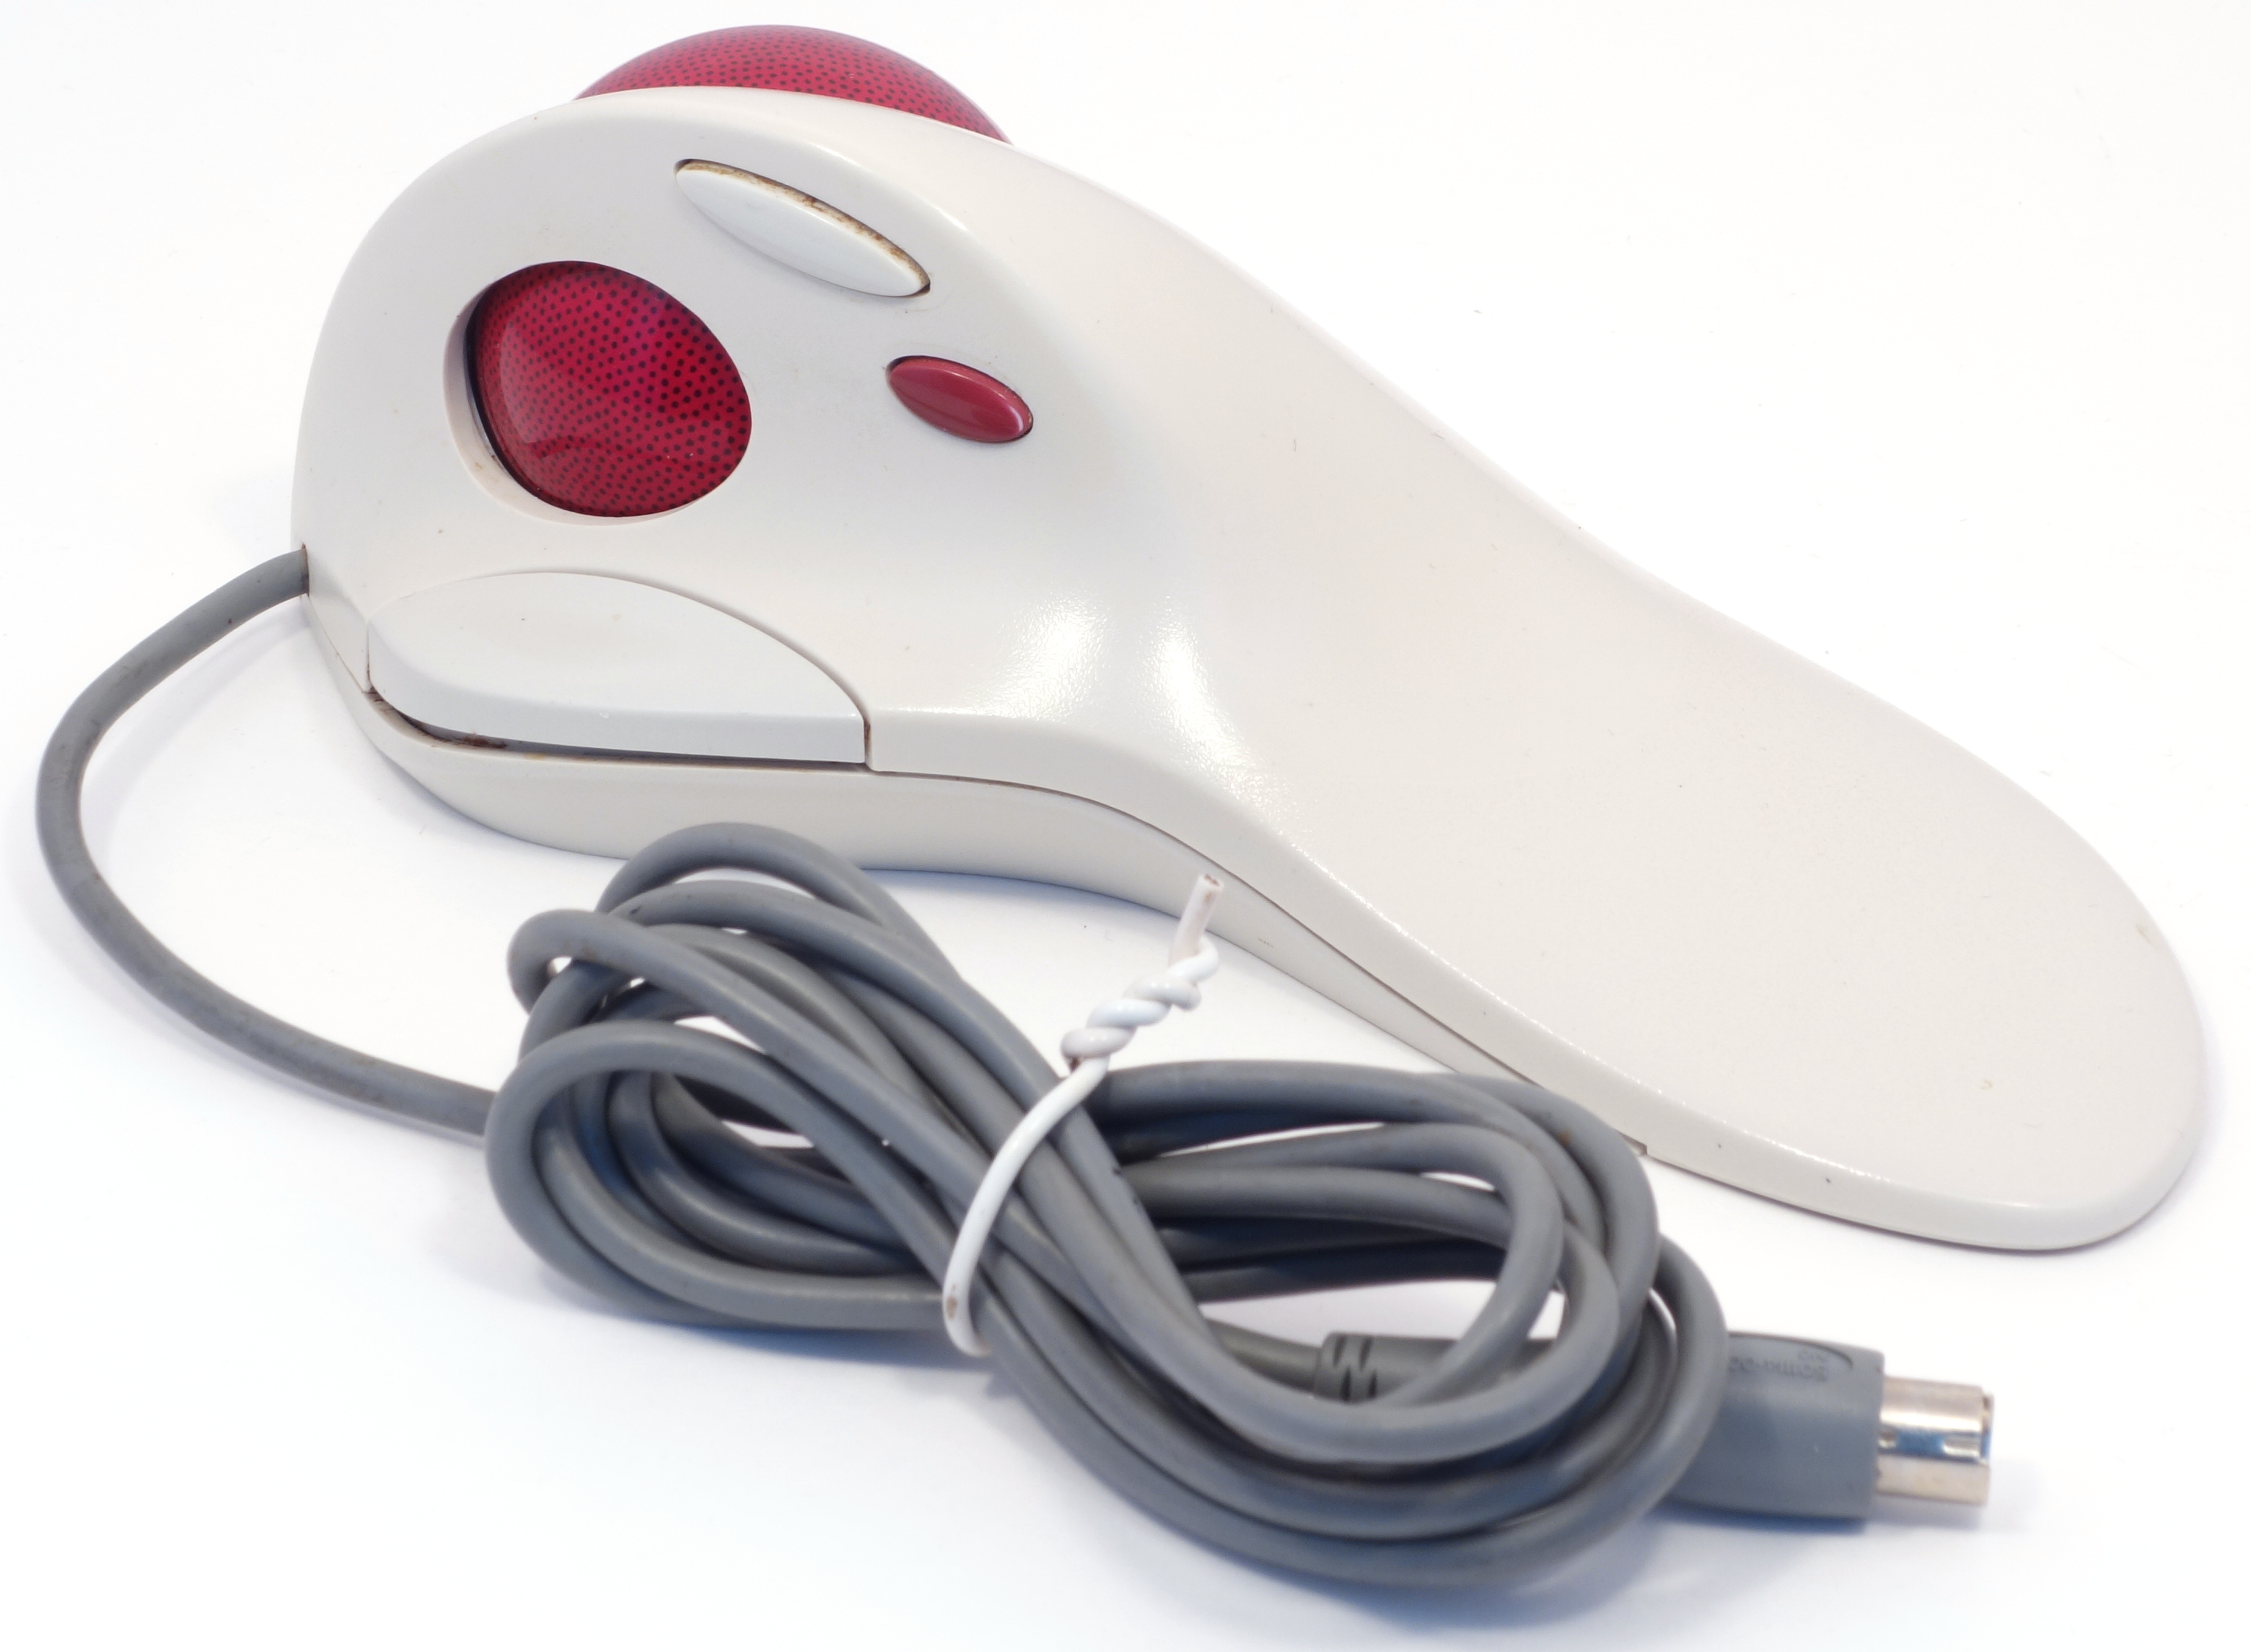
\includegraphics[scale=0.4]{1998_logitech_trackman_marble_fx/pic_30.jpg}
    \caption{Logitech TrackMan Marble FX trackball}
    \label{fig:trackman}
\end{figure}

The complex shape, which suggests thoughts of rocks altered by the long work of wind or waves, is more in the style of Luigi Colani's artistic mice and trackballs than any previous Logitech designs. The trackball turned out to be bright, memorable, and deservedly won the prestigious ``IF Design Award'' from iF International Forum Design GmbH  \cite{award}.

\begin{figure}[h]
    \centering
    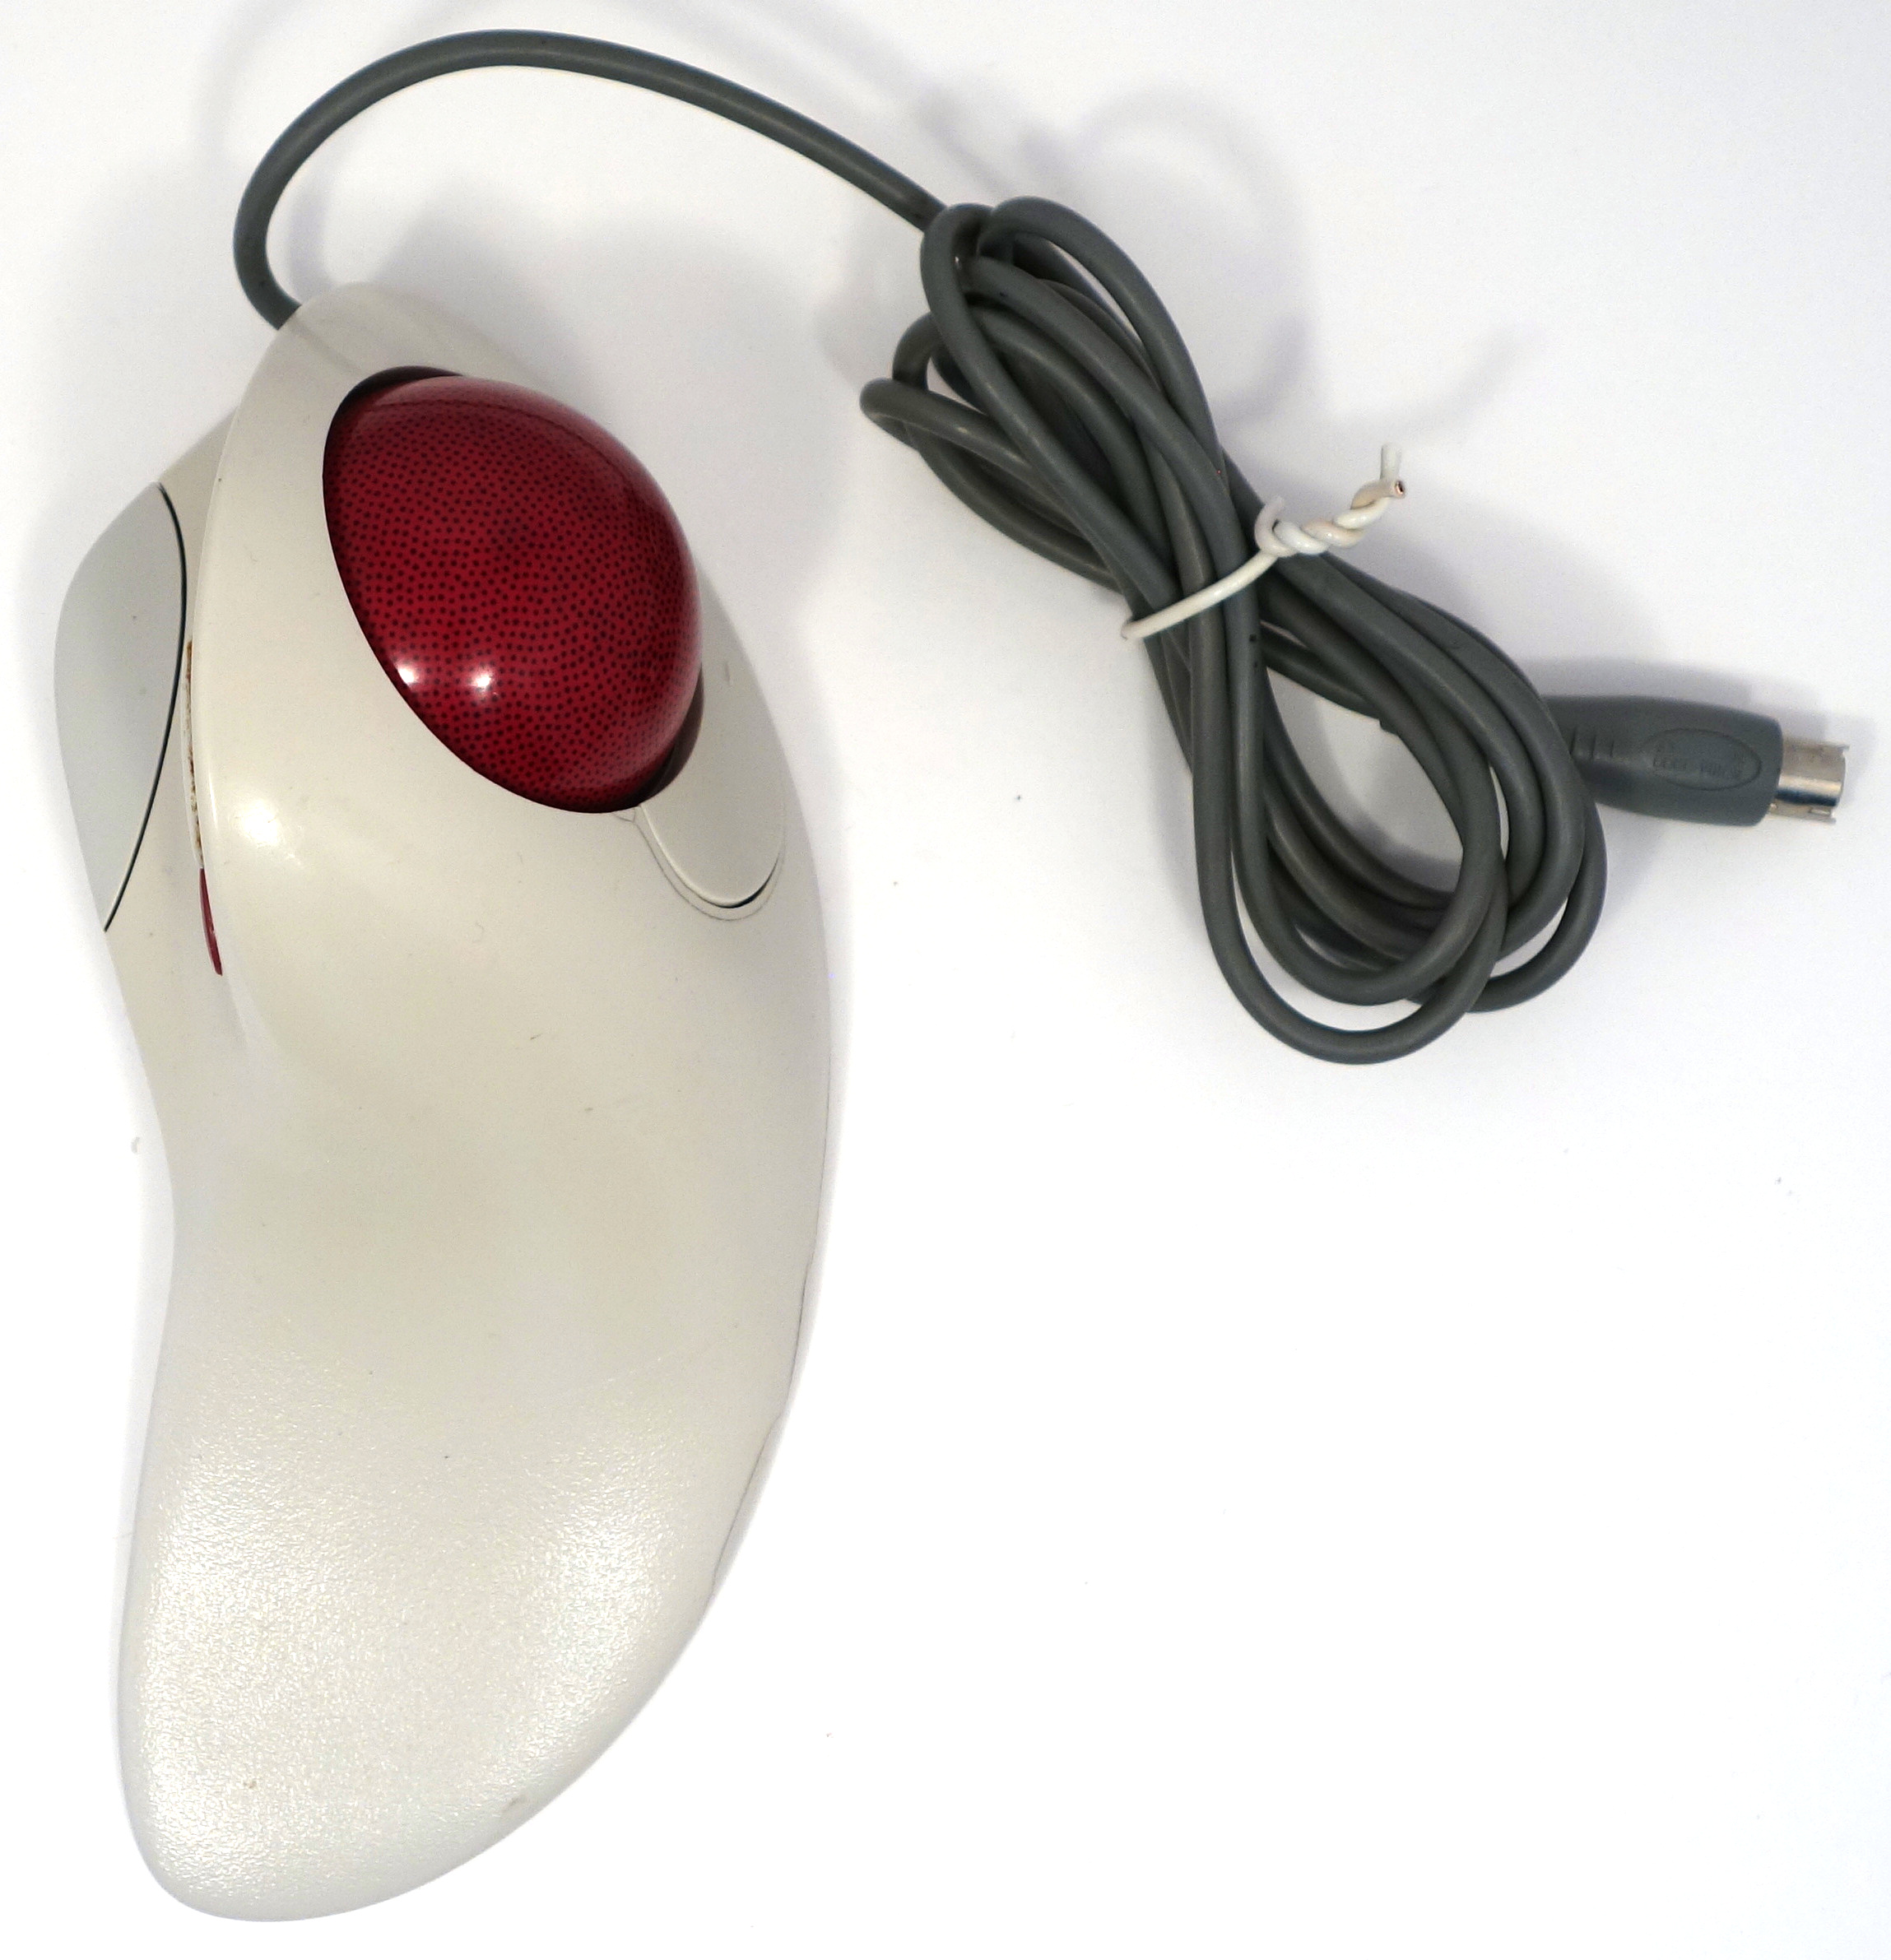
\includegraphics[scale=0.32]{1998_logitech_trackman_marble_fx/top_60.jpg}
    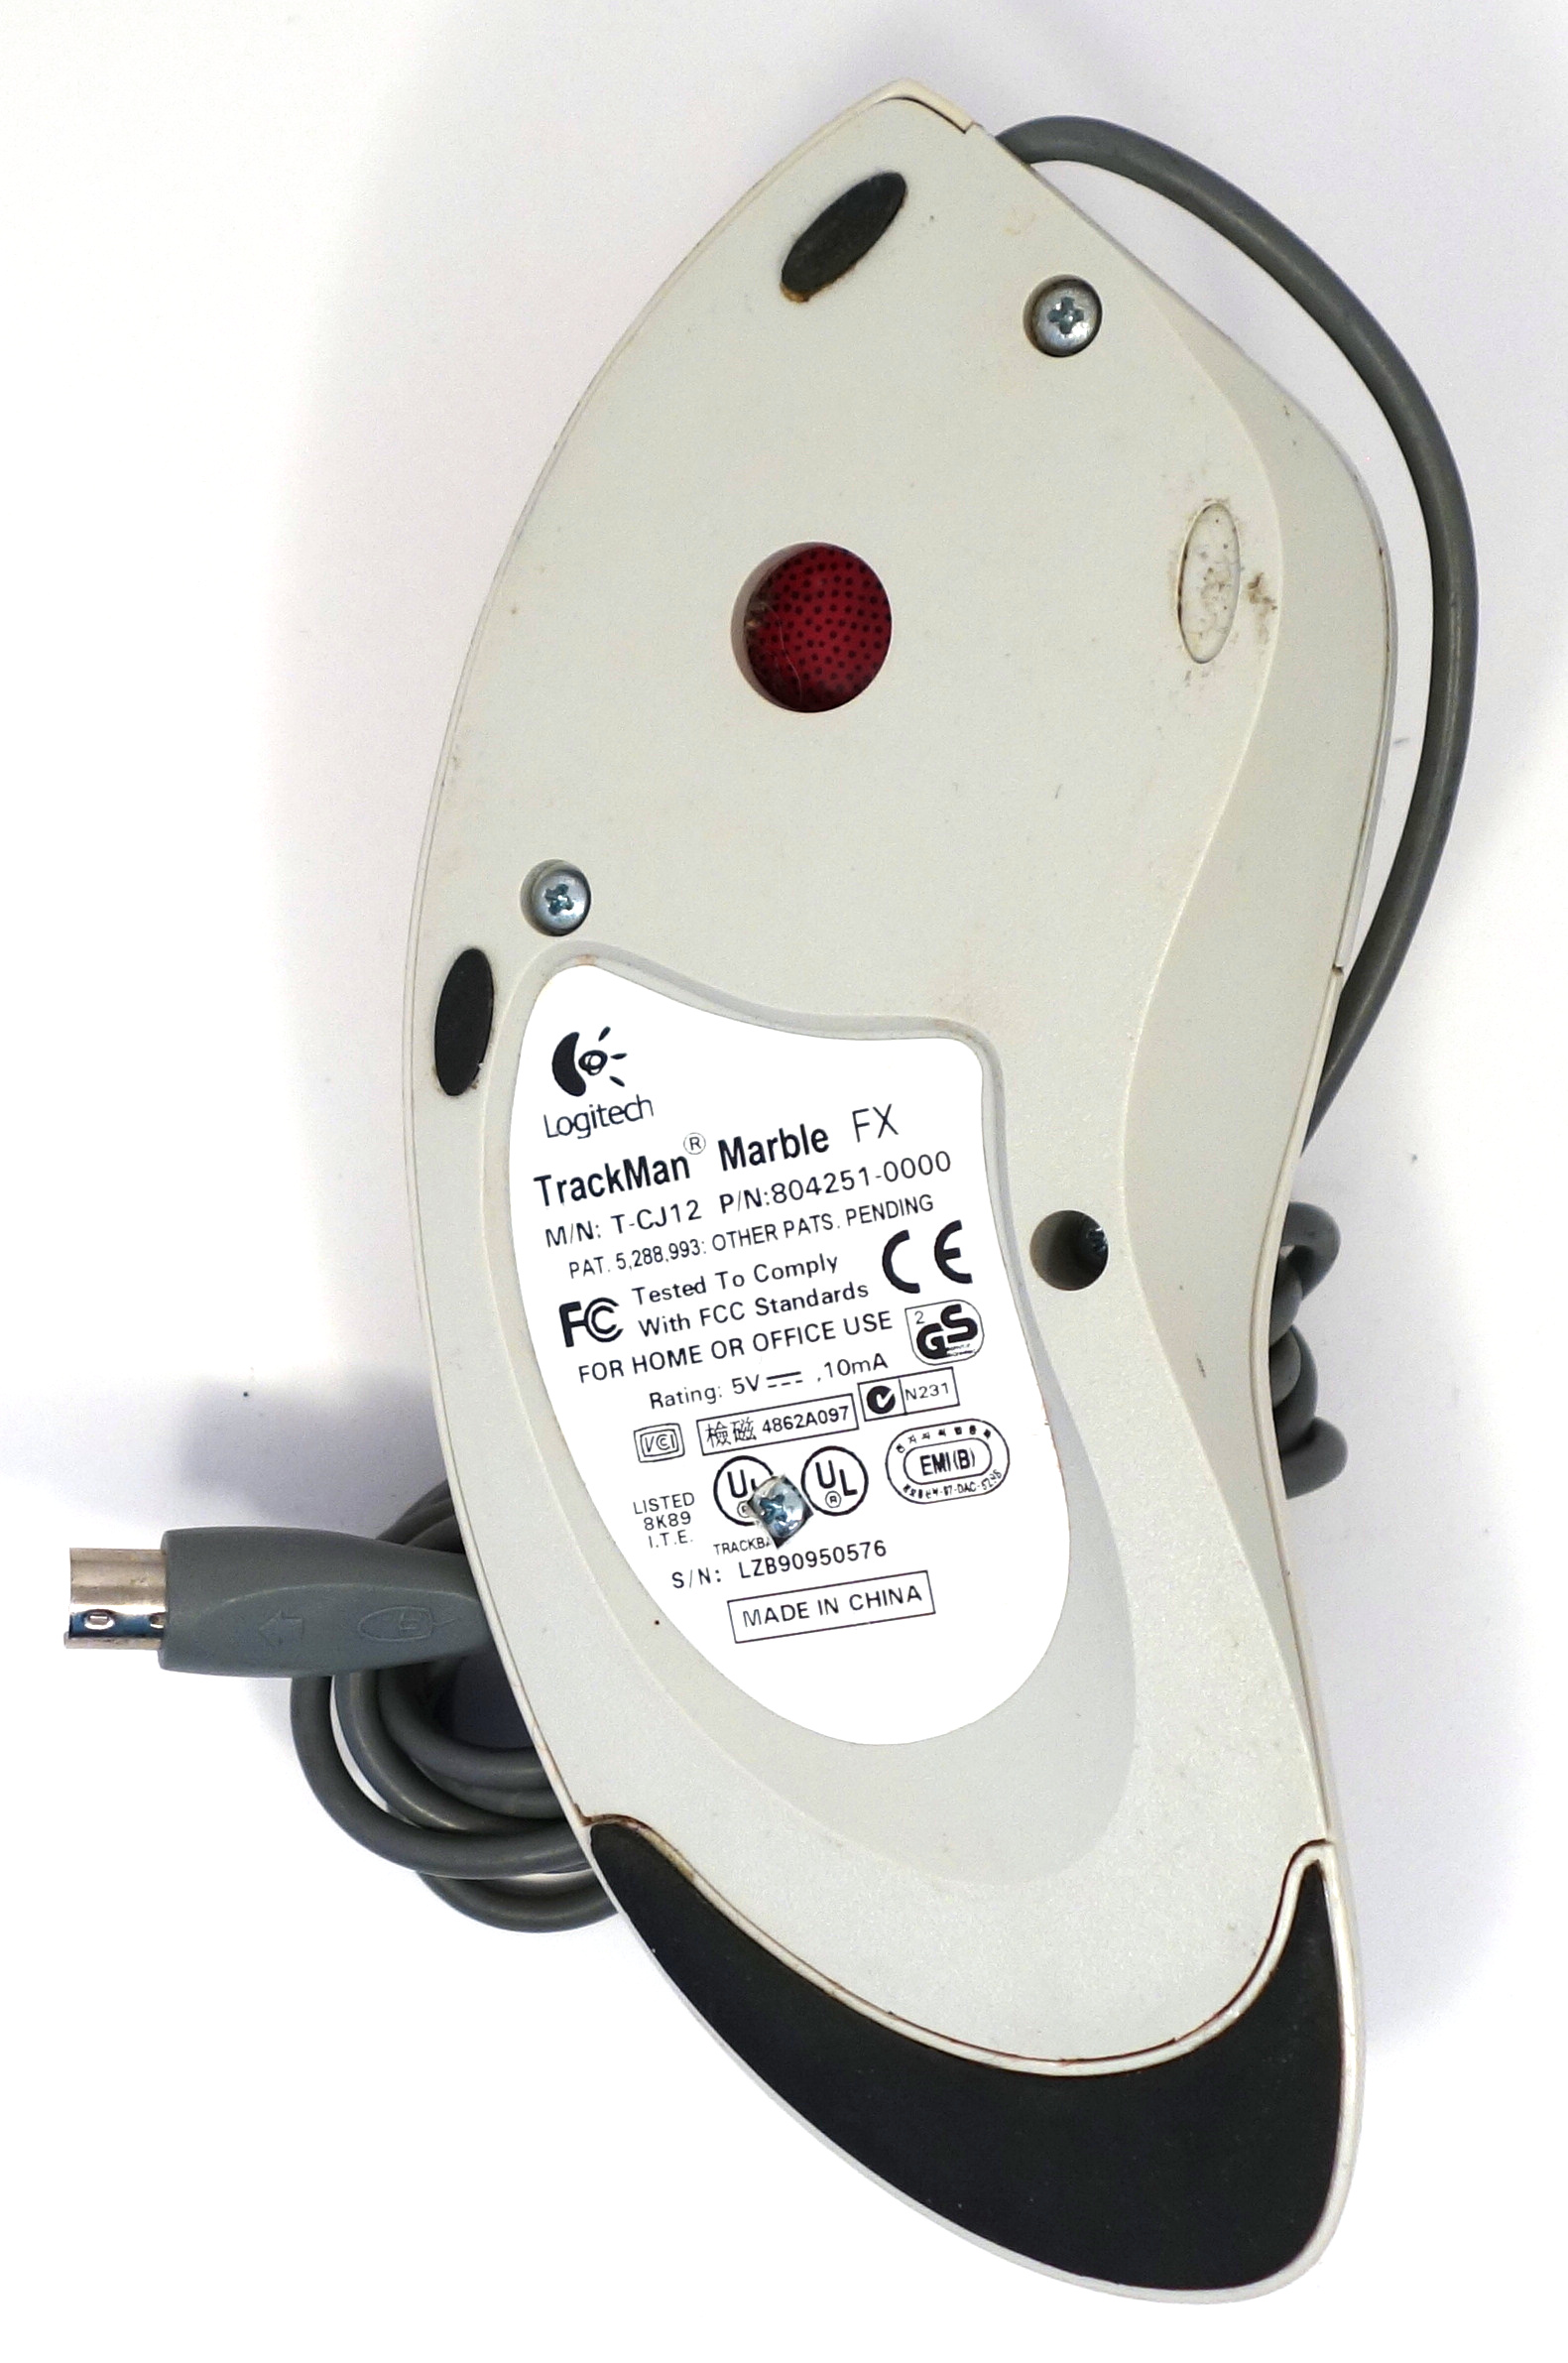
\includegraphics[scale=0.32]{1998_logitech_trackman_marble_fx/bottom_60.jpg}
    \caption{Logitech TrackMan Marble FX, top and bottom views}
    \label{fig:trackmanTopAndBottom}
\end{figure}

The TrackMan Marble FX has four keys: three on the left side of the body and one on the right (fig. \ref{fig:trackmanTopAndBottom}).
The white buttons are responsible for the standard functions of the mouse buttons, and when you click on the red button located near the ball, the driver that came with the trackball had to switch between the cursor movement mode and the scrolling/zooming mode.

A regular pattern of dark dots on the surface of the ball is needed for an optical sensor. The trackball is connected to the computer via the PS/2 interface.

\begin{figure}[h]
    \centering
    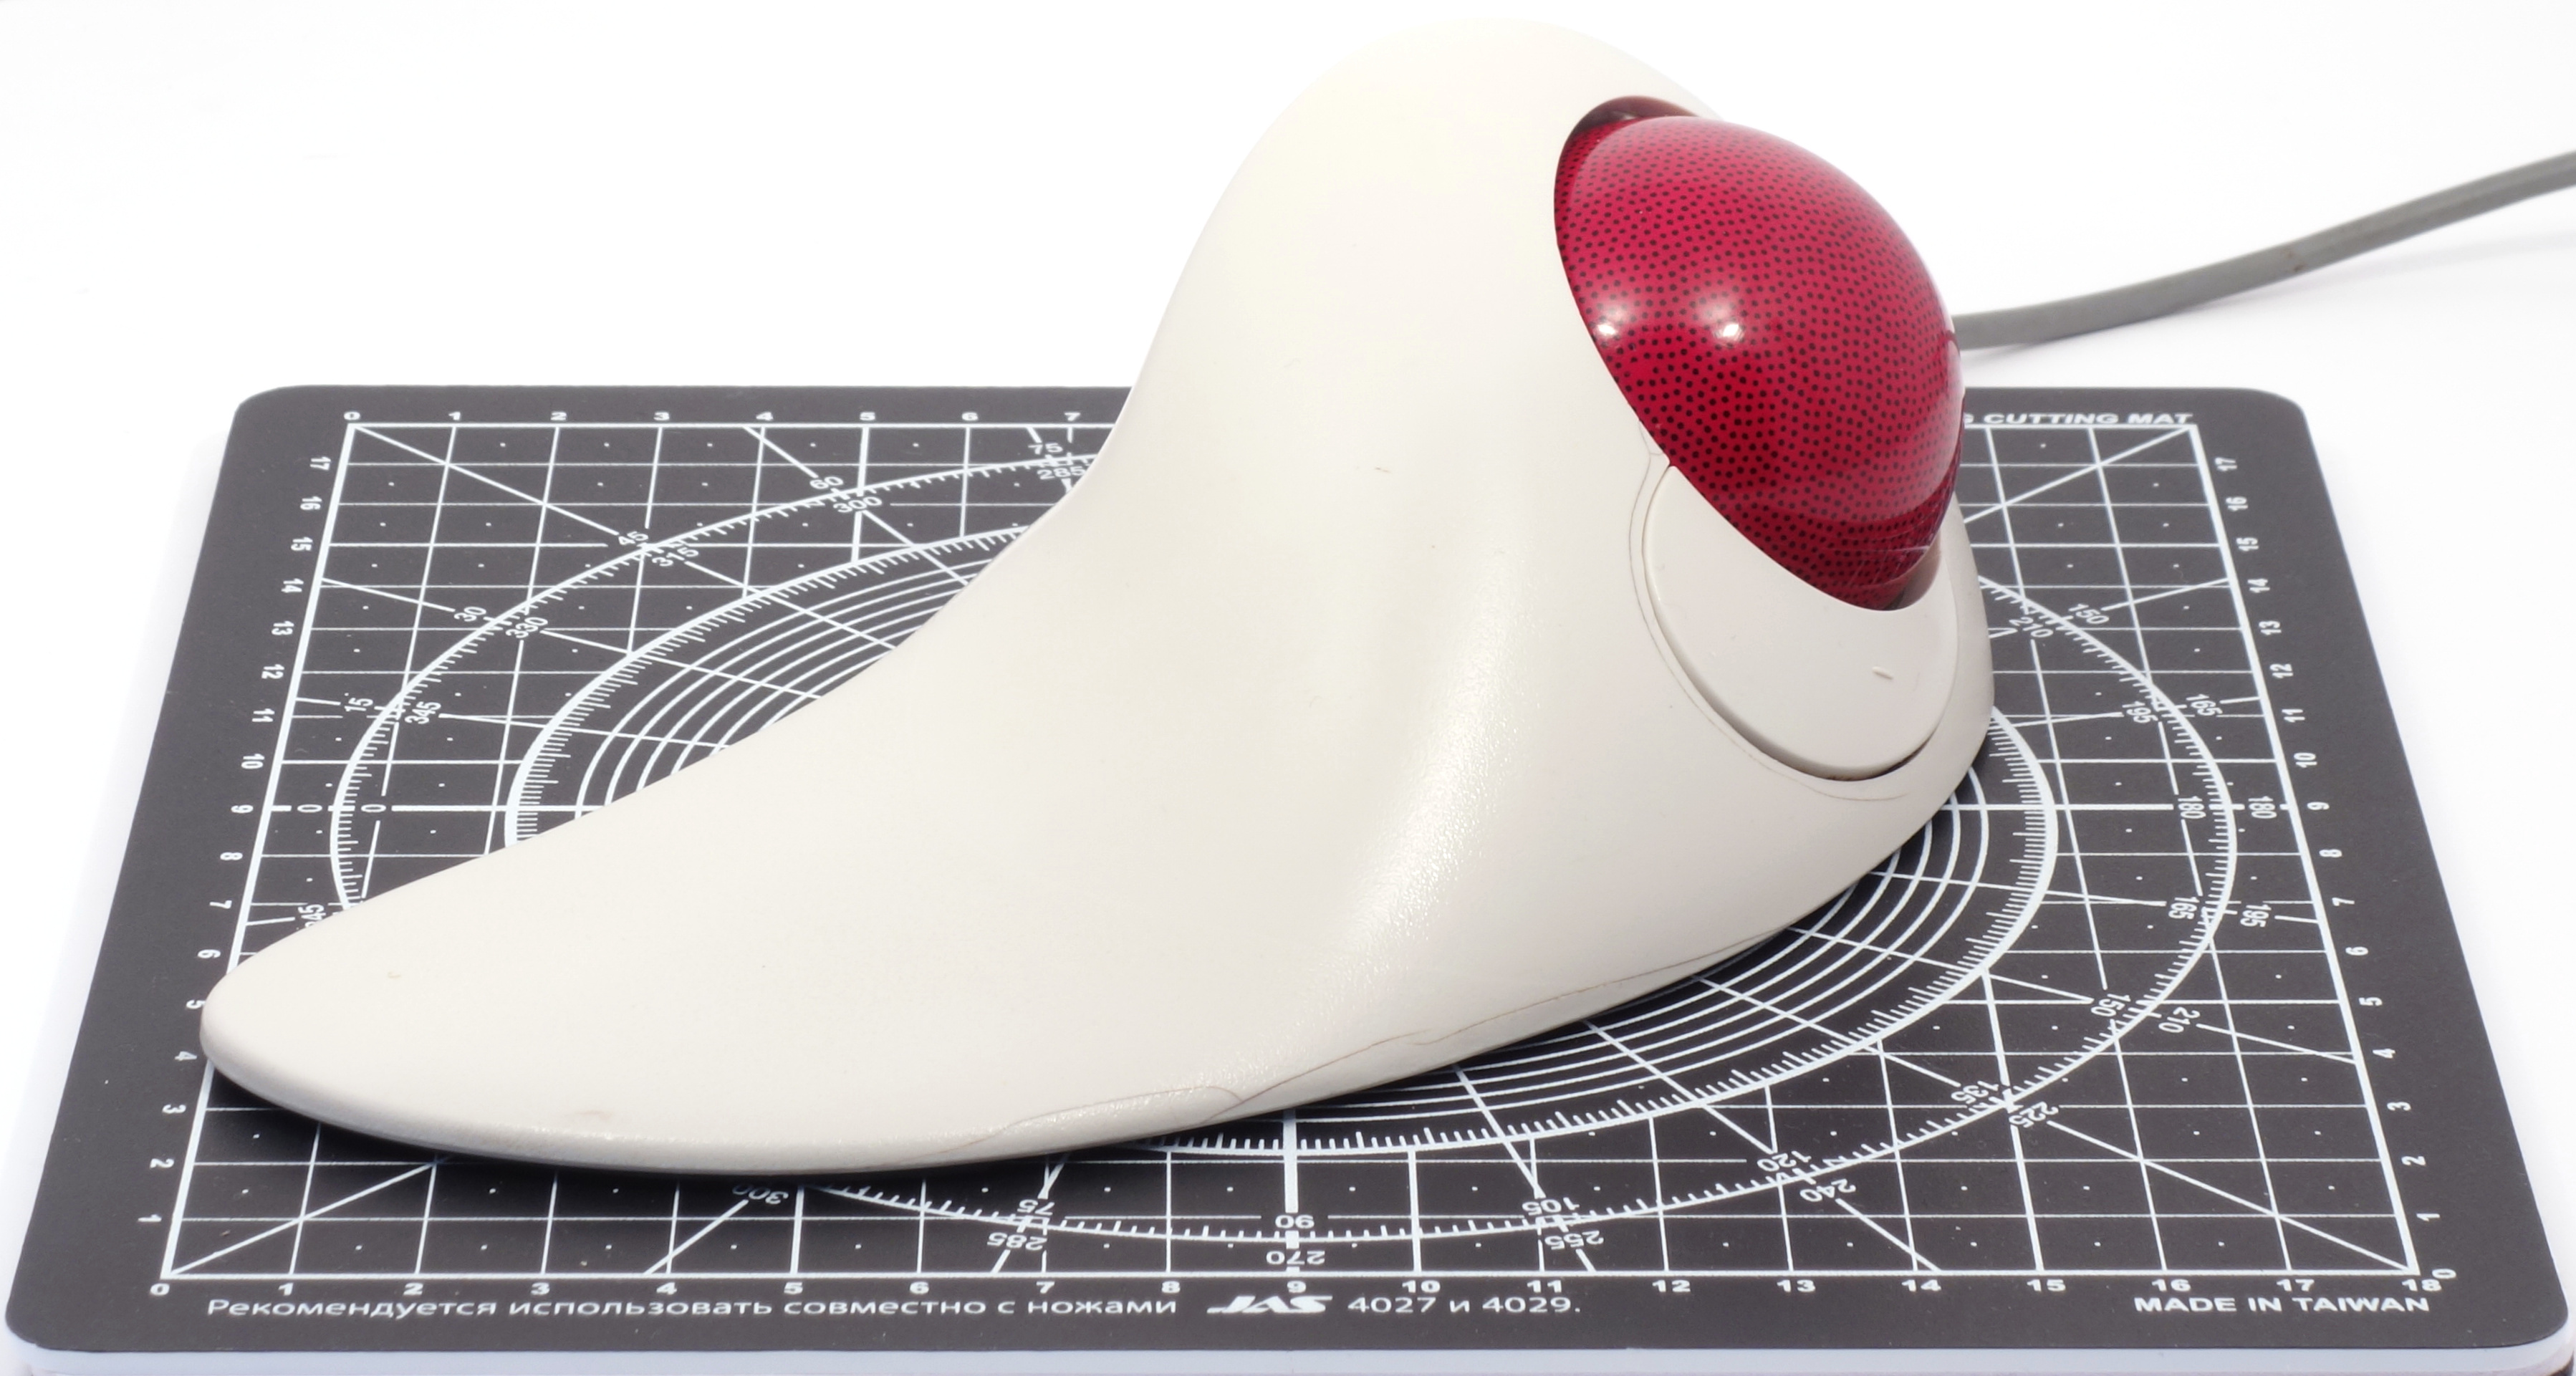
\includegraphics[scale=0.4]{1998_logitech_trackman_marble_fx/size_30.jpg}
    \caption{Logitech TrackMan Marble FX on a graduated pad with a grid step of 1~cm}
    \label{fig:trackmanSize}
\end{figure}

The TrackMan Marble FX is larger and has a larger ball than previous Logitech trackballs (fig. \ref{fig:trackmanSize}). The trackball is asymmetrical and is intended for right-handed use only, while the slope and curves of the body are designed to keep the user's wrist in the most natural position possible (fig. \ref{fig:trackmanHand}).

\begin{figure}[h]
    \centering
    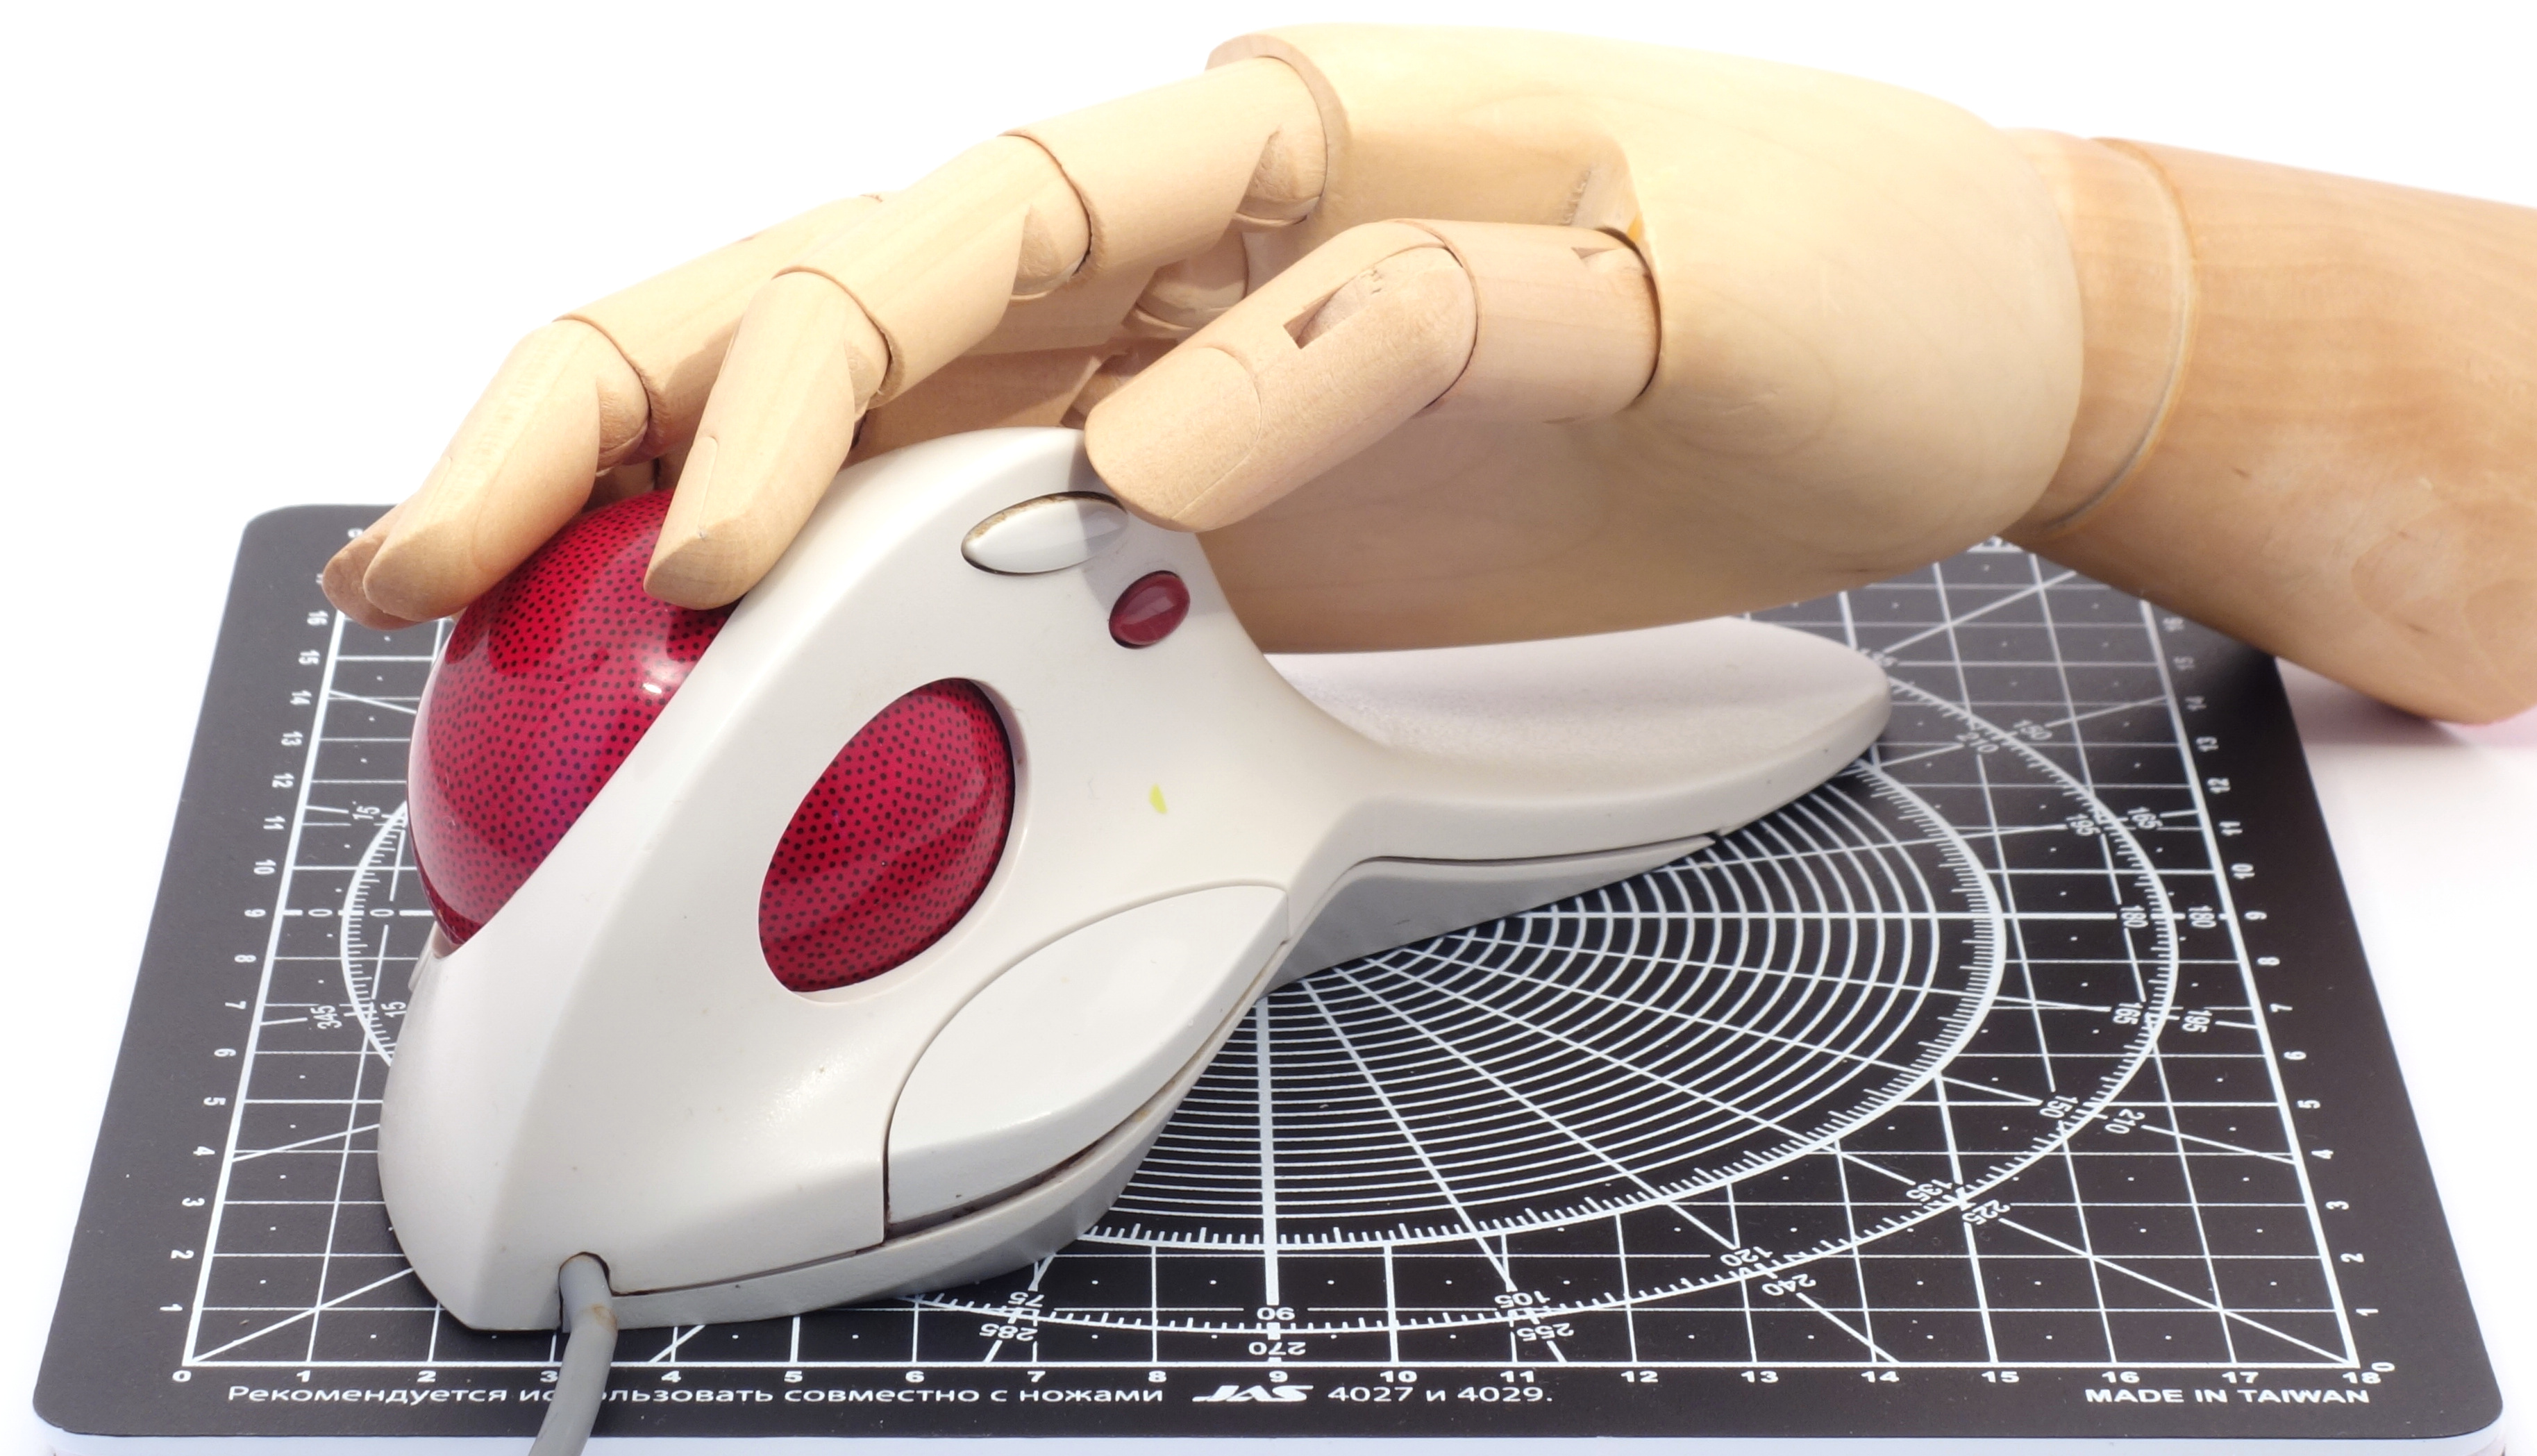
\includegraphics[scale=0.6]{1998_logitech_trackman_marble_fx/hand_30.jpg}
    \caption{Logitech TrackMan Marble FX with a human hand model}
    \label{fig:trackmanHand}
\end{figure}

Articles published in ZDNET \cite{zdnet} and in Computer Gaming World magazine \cite{gaming} noted that the TrackMan Marble FX is quite comfortable to use, but the hole in the case, designed to allow the ball to be moved with fingers from both sides, does not very suitable for this purpose due to its small size (rather, it has an aesthetic function, and also makes it easier to remove the ball from the body for cleaning). In addition, the wrist rest part of the case has received mixed reactions from some users, who would have preferred more flexibility through the use of a detachable accessory in this role.

Trackball internals are shown on figure \ref{fig:trackmanInside}. It reveals the design similar to an optical mouse that reads brightness changes using a special pad with a grid applied on it (the pattern on the ball plays the role of the grid).

\begin{figure}[h]
    \centering
    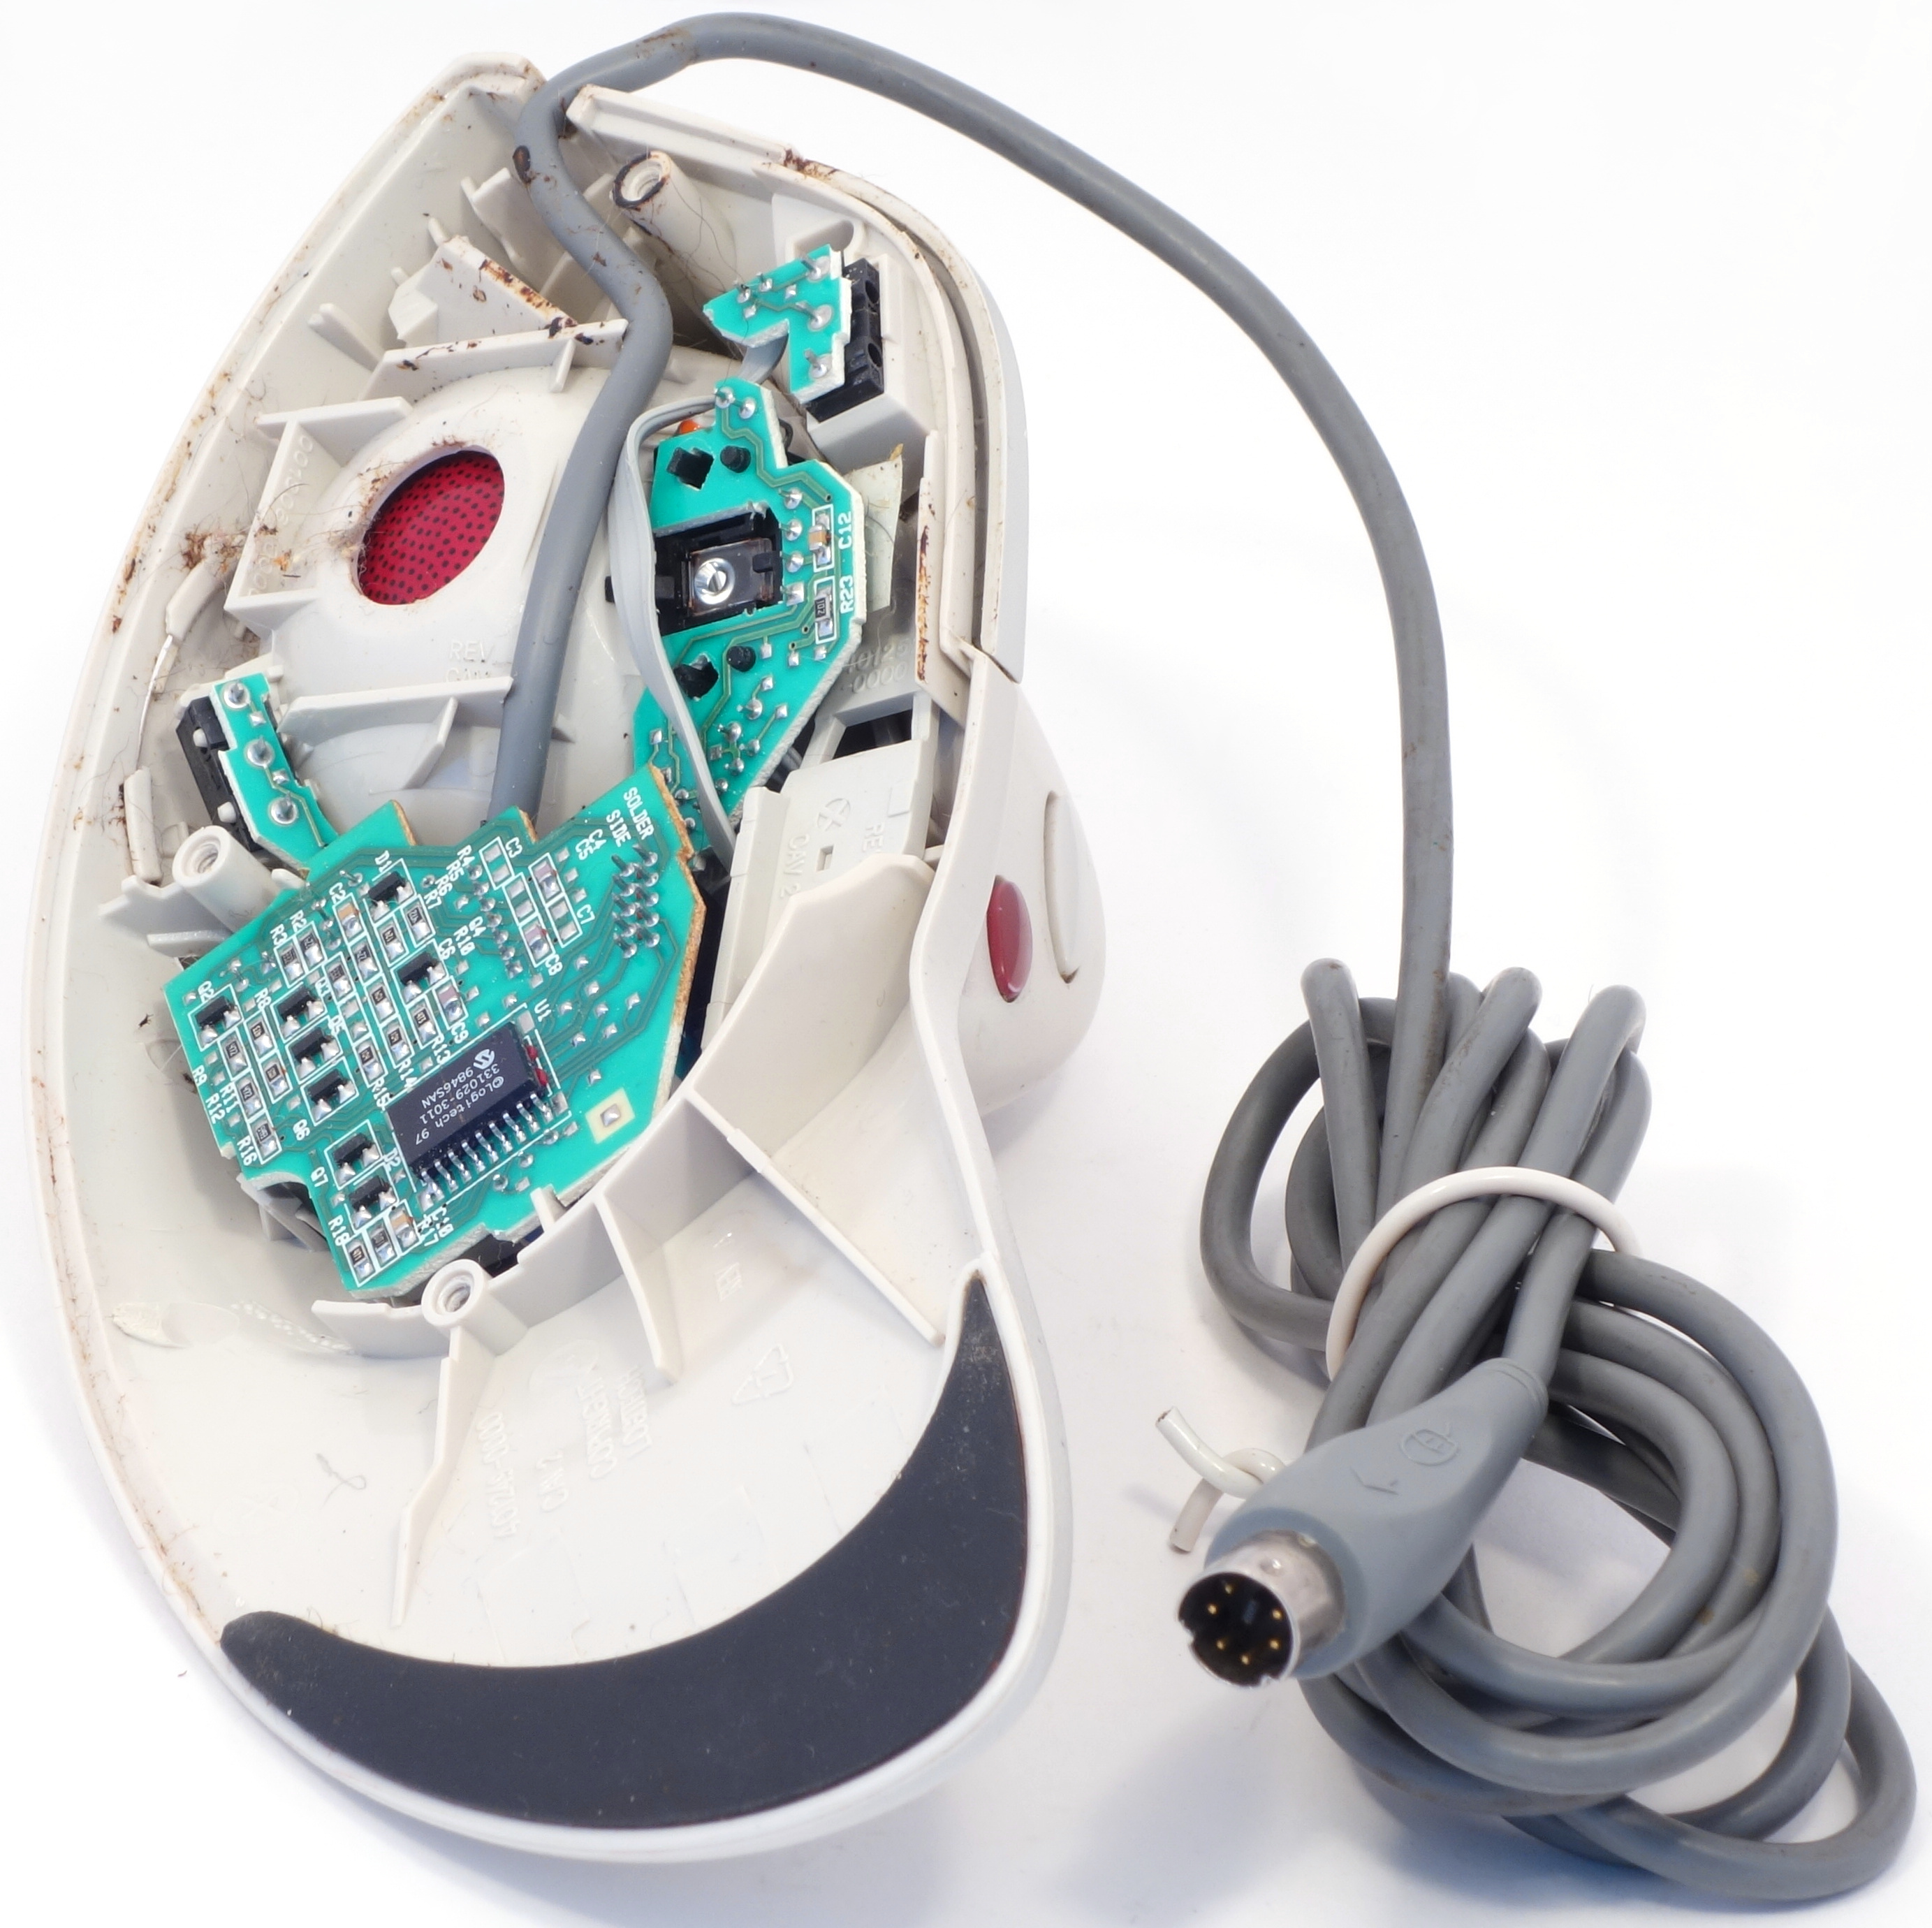
\includegraphics[scale=0.6]{1998_logitech_trackman_marble_fx/inside_30.jpg}
    \caption{Logitech TrackMan Marble FX trackball disassembled}
    \label{fig:trackmanInside}
\end{figure}

\begin{thebibliography}{9}
\bibitem{marbleBoot} Pure lust. High-tech toys and tools with the right stuff. // Boot Magazine: Issue 20 - April 1998. -- p. 18. \url{https://archive.org/details/boot-magazine-issue20-pc-notebook-autopsy-apr-1998/page/n19/mode/2up}
\bibitem{gaming} Case L. Revew - Logitech Trackman Marble/FX. Absolutely Marble-ous. // Computer Gaming World: Issue 168 - July 1998. -- p. 127.  \url{https://archive.org/details/Computer_Gaming_World_Issue_168/page/n129/mode/2up}
\bibitem {zdnet} Watson J.A. Trackballs that I have known and loved: A history in hardware. - ZDNET, March 16, 2017. \url{https://www.zdnet.com/article/trackballs-that-i-have-known-and-loved-a-history-in-hardware/}
\bibitem {award} IF Design - TrackMan Marble FX \url{https://ifdesign.com/en/winner-ranking/project/trackman-marble-fx/16939}
\end{thebibliography}

\end{document}
